\documentclass[12pt]{article}
\usepackage[english]{babel}
\usepackage{enumerate, setspace, float, stackengine}
\usepackage[hidelinks]{hyperref}
\usepackage[margin=1.5cm]{geometry}
\usepackage{caption, subcaption}
\usepackage{amsmath, amsfonts, amssymb}
\usepackage{fontspec}   %加這個就可以設定字體
\usepackage{xeCJK}       %讓中英文字體分開設置
\setCJKmainfont{標楷體} %設定中文為系統上的字型,而英文不去更動,使用原TeX字型

\title{\textbf{Theory of Computer Games}\\ Homework\#1 - Dominosa}

\author{R04922058 鄭以琳}
\date{\large \today}


\begin{document}
\maketitle

\section{Game Description}
Dominosa is a logic puzzle. It is played on a board with $(N+1)\times(N+2)$ numbers on it. Each number is an integer between $0\sim N$. The player is given $\frac{(N+1)\times(N+2)}{2}$ domino bones. Each domino is a 1*2 rectangle containing distinct pair of numbers $(i,j), 0<i\leq j\leq N$. The object is to locate all the domino bones onto the board. A bone can only be put at a location where the numbers on the bone is the same as the numbers on the board.

	\begin{figure}[H]
	\centering
	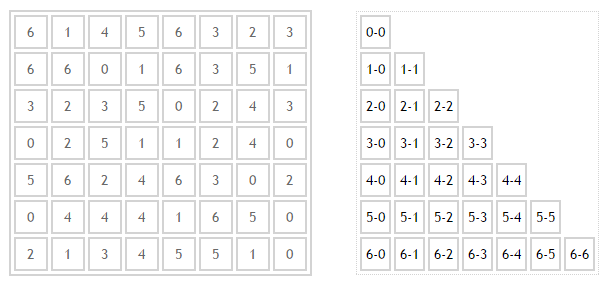
\includegraphics[width=0.6\textwidth]{fig_description1}
	\caption[Caption for the list of figures]{}
	\label{fig:description1}
	\end{figure}

Take Figure \ref{fig:description1} for example. The player is given a $(7\times8)$ board on the left and $28$ domino bones on the right. Figure \ref{fig:description2} shows one valid solution.

	\begin{figure}[H]
	\centering
	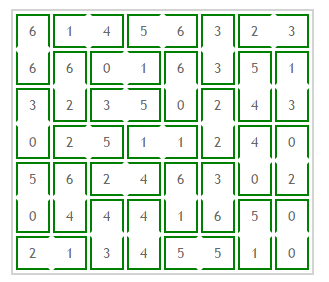
\includegraphics[width=0.3\textwidth]{fig_description2}
	\caption[Caption for the list of figures]{}
	\label{fig:description2}
	\end{figure}

Note that for an $(N+1)\times(N+2)$ board, the maximum number on the bones will be $N$ and each domino bone is used exactly once in the solution.\\

In my homework, I transformed this problem into another identical one:
\begin{quote}
Given an $(N+1)\times(N+2)$ board, two adjacent grids can be circled to form a pair. Find a way to circle each grid exactly once, and let each pair of numbers $(i,j), 0<i\leq j\leq N$ also appears exactly once.
\end{quote}

 
\section{Game Analysis}
\subsection*{Naive Brute-force Approach}
A naive searching algorithm is brute-force search, employing DFS to find every possible way of circling the numbers. Start from the top-left grid, find an uncircled adjacent grid and pair with it. In the next state, pick the first uncircled grid in row major and continue DFS. For an uncircled grid, there are at most four options to pair with, yielding a  branching factor of DFS tree $e=4$. For an $(N+1)\times(N+2)$ board, the player should circle $	\frac{(N+1)\times(N+2)}{2}$ pairs. So the depth of a solution $d=\frac{(N+1)\times(N+2)}{2}$.

Although brute-force method is guaranteed to find a solution, it's inefficient. Worst case time complexity of this algorithm is $O(e^d) = O(4^{N^2})$.

There are about $10^{12}$ different valid ways to circle the numbers on a $(10\times11)$ board (calculated by DP method). When $N$ becomes larger, the number grows dramatically. When $N=15$, there are $10^{18}$ ways, which is $10^6$ times larger than $N=9$. A pattern database may not be able to store all these options. Even with enough memory, this approach may still be very time-consuming. 	

\subsection*{Useful Properties}
	\begin{figure}[h]
		\centering
		\begin{minipage}[b]{0.3\textwidth}
			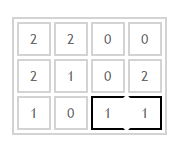
\includegraphics[width=\textwidth]{fig_forced_location}
			\caption[Caption for the list of figures]{}
			\label{fig:forced_location}
		\end{minipage}
		~
		\begin{minipage}[b]{0.3\textwidth}
			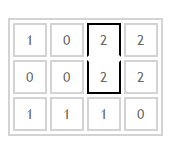
\includegraphics[width=\textwidth]{fig_invalid_circling}
			\caption[Caption for the list of figures]{}
			\label{fig:invalid_circling}
		\end{minipage}
	\end{figure}
\paragraph*{Forced Locations}
The constraint that each pair of numbers should be circled once may create some forced locations. Consider Figure \ref{fig:forced_location}, the pair $(1,1)$ can only be found at the bottom-right corner, which forced those two grids to be paired together.
	
\paragraph*{Invalid Circling}
Since every grid should be paired, if circling two grids makes another grid out of option, the circling is invalid. Take Figure \ref{fig:invalid_circling} for example - If $(2,2)$ in the third column is circled, the top-right grid can only be paired with another $2$ below, which is invalid because already exists a $(2,2)$ pair. Thus, $(2,2)$ in the third column can't be circled.

\subsection*{Possible Accelerations}
\paragraph*{Move Ordering}
Naive brute-force algorithm picks the next grid to circle in row major order. However, it will be more efficient to pick a grid with minimum branching factor first. This could reduce the chance of traversing wrong paths. In this problem, forced locations should be circled first, since its branching factor is always one. Forced locations will always be part of the solution.

\paragraph*{Eliminate Used Grids and Pairs}
After circling two grids and forming a pair, any pair associated with the two grids and the corresponding numbers should be eliminated. Consider Figure \ref{fig:eliminate}, circling the top-right pair $(0,2)$ (marked with black border) makes the other five pairs invalid (marked with red borders).
	\begin{figure}[H]
	\centering
	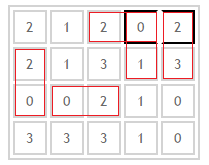
\includegraphics[width=0.3\textwidth]{fig_eliminate}
	\caption[Caption for the list of figures]{}
	\label{fig:eliminate}
	\end{figure}
Set counters to maintain the remaining count of valid options for each unused grids and pairs. They can be useful for deciding the move ordering.

\paragraph*{Detect Invalid Moves}
As discussed in the prior section, invalid circling can never lead to a solution. If those invalid moves can be detected earlier, states that are not likely leading to the goals will not be explored further. A way to do so is to check whether every unused grid and unused pair has at least one option after a move.

\section{Problem Transformation}
\subsection*{Exact Cover Problem}
This problem can be transformed into another well-known problem called "Exact Cover Problem":
\begin{quote}
	Given a set $X$ and a collection of subsets $S=\{S_1,S_2,\cdots S_n\}$, an exact cover is a set $S^*\in S, s.t.$ each element in $X$ is contained in exactly one subset in $S^*$.
\end{quote}
The set $X$ in Dominosa is a set containing every grid and every possible pair of numbers. $S$ is a set containing the choices of circling. Each subset in $S$ can be represented by two grids $(r1, c1),(r2,c2)$ and their corresponding numbers $(v1,v2)$.

The goal of this problem is to find a subset in $S$ (i.e. find a way of circling) s.t. every grid and every pair is used exactly once.

\subsection*{Knuth's Algorithm X}
Donald Knuth presented an algorithm named Algorithm X to solve the exact cover problem. The problem is represented using a matrix $A$ consisting of 0s and 1s. Each column represents an element in $X$. Each row represents a subset in $S$. The goal is to select a subset of rows so that the digit 1 appears in each column exactly once.

This is a recursive algorithm. Main concepts are stated below:
\begin{enumerate}
	\item If A contains no columns, terminate successfully.
	\item Otherwise, choose a column $c$.
	\item For each row $r$ that $A_{r,c}=1$
	\begin{enumerate}
		\item Delete each column $j$ and each row $i$ in $A$, where $A_{r,j}=1$ and $A_{i,j}=1$.
		\item Solve matrix $A$ recursively.
		\item If a solution is found, add $r$ to the solution and return.
	\end{enumerate}
\end{enumerate}

\subsection*{Dancing Links}
In order to solve the exact cover problem, Knuth also presented a data structure "Dancing links". Using a naive implementation to store matrix $A$ will spend lots of time searching for $1s$. Therefore, Knuth implemented a sparse matrix where only $1s$ are stored. Each node in the matrix represents an $1$, and each node points to its four adjacent nodes. Consider Figure \ref{fig:dl}, instead of storing the exact matrix on the left, use 2D doubly linked list on the right to represent the matrix.
	\begin{figure}[H]
	\centering
	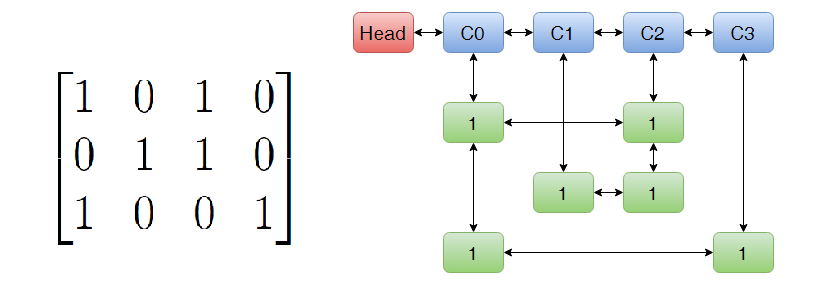
\includegraphics[width=0.6\textwidth]{fig_dl}
	\caption[Caption for the list of figures]{}
	\label{fig:dl}
	\end{figure}
This method can improve the search time complexity from $O(n)$ to $O(1)$.

\section{Implementation Details}
I implemented Algorithm X and dancing links in my homework. Given Figure \ref{fig:imp_init} as initial board, $(0,0)$ is the top-left grid, some implementation details are discussed below.
	\begin{figure}[H]
	\centering
	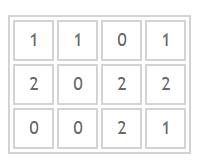
\includegraphics[width=0.2\textwidth]{fig_imp_init}
	\caption[Caption for the list of figures]{}
	\label{fig:imp_init}
	\end{figure}

\subsection*{Data Structure}
	\begin{figure}[H]
	\centering
	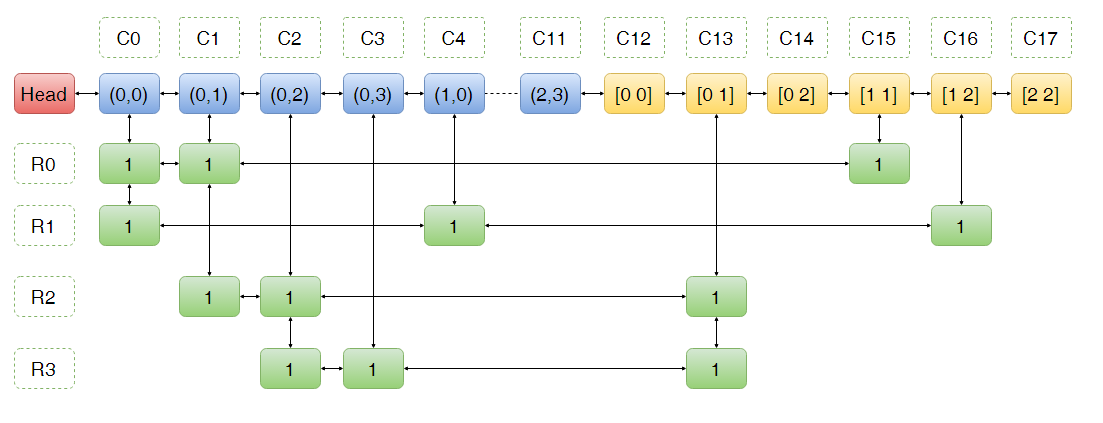
\includegraphics[width=0.9\textwidth]{fig_imp_ds}
	\caption[Caption for the list of figures]{}
	\label{fig:imp_ds}
	\end{figure}
Figure \ref{fig:imp_ds} shows a part of the dancing links corresponding to the initial board. Blue columns ($C_0$ -- $C_{11}$) represent the grids. Yellow columns ($C_{12}$ -- $C_{17}$) represent the pairs.

Each row represents an option of circling, so each of them contains exactly three $1s$. For example, $R0$ means circling grids $(0,0)$ and $(0,1)$ can form a pair $(1,1)$; $R1$ means circling grids $(0,0)$ and $(1,0)$ can form a pair $(1,2)$.
There are $2RC-R-C$ pairs can be circled on an $R\times C$ board. Row count of the initial dancing links is $2RC-R-C$.

The goal is to find a collection of rows, so that each column has exactly one 1.

\subsection*{Algorithm}
Recursively solve the problem by DFS method. In each stage, search for a column $c$ with minimum number of $1s$. In this example, $C4$ is most likely to be chosen.

For the chosen column $c$, arbitrarily pick a row $r$ which has an $1$ in column $c$. $R1$ is the only candidate here. Note that if there are multiple choices, pick any one and continue DFS. If in further states, the algorithm failed to find a solution, it will return to this stage and try another row.

\subsection*{Eliminate Collisions}
After choosing a row $r$, the rows containing collision $1s$ need to be removed. Choosing $R1$ to be part of the solution means that we formed a pair $(1,2)$ by circling grids $(0,0)$ and $(1,0)$. Therefore, any other choices containing those two grids or the pair should be removed. There is only one row $R0$ needs to be removed in this example. Since column $c$ is already covered by the choice, it will also be removed.

The remaining state is illustrated in Figure \ref{fig:imp_remove}.

	\begin{figure}[H]
	\centering
	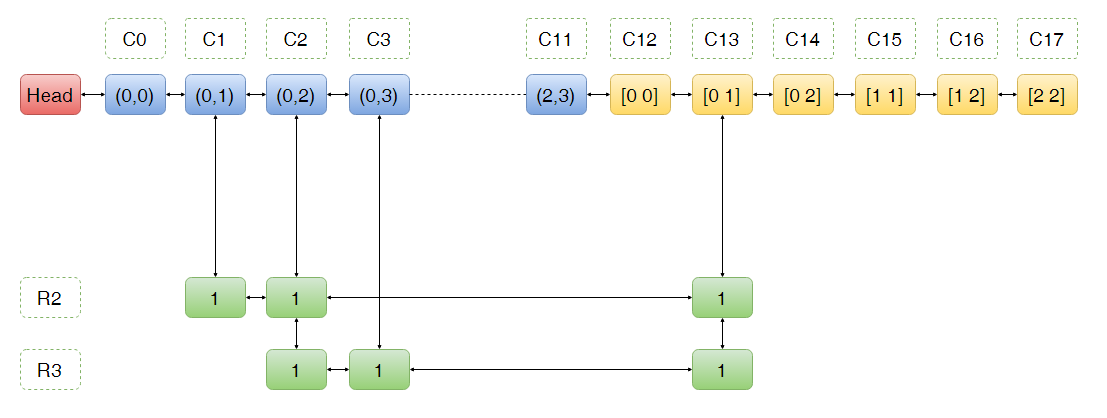
\includegraphics[width=0.9\textwidth]{fig_imp_remove}
	\caption[Caption for the list of figures]{}
	\label{fig:imp_remove}
	\end{figure}
	
\subsection*{Detect Invalid moves}
If removing a column and some rows after a choice leaving another column $c'$ with no $1s$, this choice can never lead to a solution because $c'$ will not be covered. In this case, algorithm should choose another option or return to the prior state (if there are no other options).

\subsection*{}
If the input is a valid board, the algorithm will terminate successfully and return the answer.

\section{Experiment and Analysis}
The websites I used to generate boards are listed below:
\begin{itemize}
	\item \url{http://www.puzzle-dominosa.com/}
	\item \url{http://www.chiark.greenend.org.uk/~sgtatham/puzzles/js/dominosa.html}
	\item \url{http://coderazzi.net/javascript/dominosa/dominosa.html}
\end{itemize}

\subsection*{Branching Factor}
The minimum branching factor at every state will not exceed four. This is because each grid can have at most four other grids to be paired with. Moreover, since the algorithm removes collision rows at every state, the branching factor decreases quickly.

Although some columns may have lots of $1s$ at initial state, the algorithm chooses the one with minimum options. I ran some experiments recording the minimum number of $1s$ in remaining columns at each state, and it turns out that the minimum number is never greater than two. In lots of cases, the minimum number is always one, which means DFS can always find the correct path.

I think it's because this game is originally designed for humans. Designers will often give players some good options to start with. Otherwise, the game will be too difficult to solve.

I randomly generated five $31\times 32$ boards. There are $\frac{31\cdot 32}{2}=496$ pairs need to be circled, so the answer will be at $496^{th}$ layer. Table \ref{tbl:branch_factor} shows the result of my experiment. 

\begin{table}[H]
	\centering
	\begin{tabular}{|c|c|c|c|c|c|}
	\hline
	Board ID                                      & \# 1   &\# 2   &\# 3   &\# 4   &\# 5      \\ \hline
	\# States traversed before finding a solution & 4977 & 644  & 989  & 496  & 157315 \\ \hline
	\# Minimum options \textgreater1              & 166  & 6    & 26   & 0    & 4796   \\ \hline
	Runtime (seconds)                             & 0.14 & 0.02 & 0.03 & 0.04 & 3.2    \\ \hline
	\end{tabular}	
	\caption{}
	\label{tbl:branch_factor}
\end{table}

Since the minimum number of $1s$ is less than or equal to $2$, DFS seldom needs to return and try another choice. In these five cases, program halts successfully in less than 5 seconds.

Board \# 4 is the optimal case. It could find a state with only one option at every layer, so after traversing for $496^{th}$ layers, a solution is found.

\subsection*{Move Ordering}
Another experiment I did is to pick an arbitrary column at each state instead of always choosing the one with minimum number of options. The result is shown in Table \ref{tbl:move_ordering}

% Please add the following required packages to your document preamble:
% \usepackage{graphicx}
\begin{table}[H]
\centering
\begin{tabular}{|c|c|c|c|c|}
\hline
Board ID                                                                                                             & \#1  & \#2    & \#3              & \#4                \\ \hline
N                                                                                                                    & 5    & 10     & 15               & 30               \\ \hline
\begin{tabular}[c]{@{}c@{}}\# States traversed before finding a solution\\ (Choose the optimal column)\end{tabular}  & 21   & 129    & 136              & 4977             \\ \hline
\begin{tabular}[c]{@{}c@{}}\# States traversed before finding a solution\\ (Choose an arbitrary column)\end{tabular} & 192  & 305058 & -                & -                \\ \hline
\begin{tabular}[c]{@{}c@{}}Runtime (seconds)\\ (Choose the optimal column)\end{tabular}                              & 0.01 & 0.01   & 0.01             & 0.14             \\ \hline
\begin{tabular}[c]{@{}c@{}}Runtime (seconds)\\ (Choose the optimal column)\end{tabular}                              & 0.01 & 0.2    & \textgreater5min & \textgreater5min \\ \hline
\end{tabular}

\caption{}
\label{tbl:move_ordering}
\end{table}

When $N\geq 15$, without move ordering optimization, a solution can not be found in five minutes. Table \ref{tbl:move_ordering} shows the importance of choosing a good path to DFS.

\section{Screenshot}
	\begin{figure}[H]
	\centering
	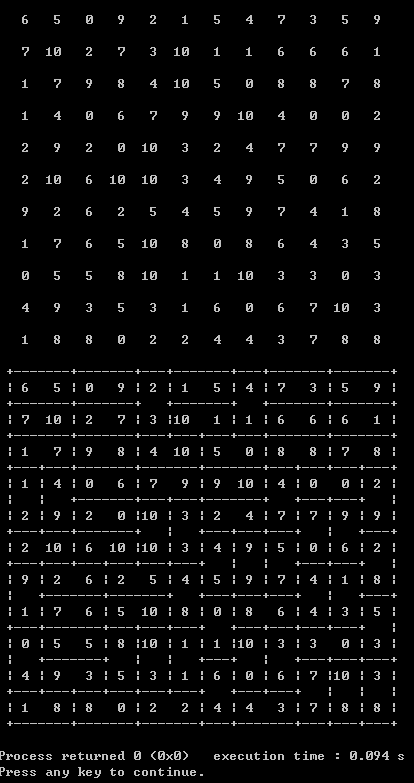
\includegraphics[width=0.5\textwidth]{fig_screen_10}
	\caption[Caption for the list of figures]{N=10}
	\label{fig:screen_10}
	\end{figure}


\begin{thebibliography}{9}

\bibitem{}
	\url{http://www.mathematica-journal.com/2014/10/three-ways-to-solve-domino-grids/}
\bibitem{}
	\url{http://11011110.livejournal.com/128249.html}
\bibitem{}
	\url{http://mypaper.pchome.com.tw/zerojudge/post/1325718060}
\bibitem{}
	\url{http://www.cnblogs.com/grenet/p/3145800.html}
  

\end{thebibliography}

 
\end{document}
